\chapter{Architettura}

Questo capitolo illustra il funzionamento e la struttura delle architetture software, sia per quanto riguarda il \gls{frontend} che il \gls{backend} di \projectName. Dal momento che entrambe le applicazioni \angular~e \nodejs~operano sugli stessi oggetti, le loro definizioni risiedono in un pacchetto \gls{npm} condiviso che esporta tutte le entità necessarie, in modo da riutilizzare il codice e renderlo facilmente manutenibile. Le principali entità esportate sono:
\begin{itemize}
	\item \textit{User}: rappresenta un utente del sistema con uno specifico ruolo
	\item \textit{Company}: rappresenta un'azienda
	\item \textit{Internship}: rappresenta un'offerta di tirocinio di un'azienda
	\item \textit{InternshipProposal}: rappresenta una proposta di candidatura di uno studente per un tirocinio
\end{itemize}

\section{Architettura lato server}

Il \gls{backend} di \projectName~è un'applicazione \nodejs~che si appoggia sul \gls{framework} \expressjs~per l'esposizione di \acrshort{rest} \acrshort{api} che interagiscono con \mongodb~attraverso l'\acrshort{orm} \mongoosejs. 
L'infrastruttura è divisa in livelli con responsabilità diverse che verranno discussi nei paragrafi seguenti.

\subsection{Schemas}

Gli \textit{schemas} sono il livello più vicino al database, essi definiscono la struttura dei documenti delle collezioni.

Pur utilizzando \mongodb~che è uno \textit{schema-less} database, infatti, ho preferito appoggiarmi su un sistema che mi permettesse di validare i dati e la loro struttura. Per fare ciò ho utilizzato \mongoosejs, un \gls{orm} che mi permette di definire la struttura dei documenti nelle collezioni del database e mi fornisce metodi di validazione e manipolazione basati su oggetti.

Gli \textit{schemas} sono la definizione dei documenti delle collezioni del database come previsti da \mongoosejs. Essi contengono la definizione del documento, dei suoi campi e del loro tipo.
% File
\begin{figure}[!h] 
	\centering    
	\lstinputlisting{Chapter2/schema.ts}
	\caption[Esempio di \textit{schema} dell'applicazione \gls{backend}]{Esempio di \textit{schema} dell'applicazione \gls{backend}}
	\label{fig:server-schema}
\end{figure}
Possiamo notare che in figura \ref{fig:server-schema}, all'interno della definizione della struttura del documento, vi sono tre proprietà --- \textit{attendances, internship e status}. Ognuno dei campi ha tipo diverso:
\begin{itemize}
	\item \textit{attendances} è un array di oggetti con una proprietà \textit{date} di tipo \textit{Date} obbligatoria
	\item \textit{internship} è una referenza di un altro schema (Internship), che verrà popolato automaticamente in fase di lettura (effettua un \gls{sqljoin} in automatico con il plugin \acrshort{npm} `mongoose-autopopulate`)
	\item \textit{status} è semplice numero
\end{itemize}
Nel caso l'applicazione cerchi di salvare un oggetto che non rispetti i vincoli imposti dallo \textit{schema} viene sollevata un'eccezione che impedisce di rendere inconsistente il database.

\subsection{Repositories}
I \textit{repositories} sono classi legate ad uno specifico \textit{schema} che esportano operazioni su di esso. Interrogano il proprio \textit{schema} per leggere, scrivere o aggregare dati e contengono solamente la logica di accesso ai dati, senza nessuna logica di business (ad esempio il controllo dei permessi).
% File
\begin{figure}[!h] 
	\centering    
	\lstinputlisting{Chapter2/repository.ts}
	\caption[Esempio di \textit{Repository}]{Esempio di \textit{repository} dell'applicazione \gls{backend}}
	\label{fig:server-repository}
\end{figure}
Tutti i \textit{repositories} derivano dal \textit{BaseRepository} che esporta le operazioni di base --- \gls{crud} --- oltre che un metodo per eseguire query personalizzate.
Ogni \textit{repository} può esporre ulteriori metodi custom ed eventualmente accedere ad altri \textit{repositories} iniettati dal sistema di \acrfull{di}. Il sistema di \acrshort{di} adottato dal sistema si basa sul pacchetto \acrshort{npm} `inversisy`, che fornisce anche un modo per aggirare le dipendenze circolari (ad esempio tra due \textit{repositories}) tramite un meccanismo di \textit{lazy-inject}.

\subsubsection{Lista \textit{repositories} pubblici}
I \textit{repositories} presenti nell'applicazione server sono:
\begin{itemize}[itemsep=0pt]
	\item \textit{CompaniesRepository}
	\item \textit{InternshipProposalsRepository}
	\item \textit{InternshipsRepository}
	\item \textit{RolesRepository}
	\item \textit{UsersRepository}
\end{itemize}
ognuno dei quali si occupa di una singola entità ed interagisce con un singolo \textit{schema}. 
\pagebreak
\subsection{Controllers}
\label{server:controllers}
I \textit{controllers} espongono su architettura \acrshort{rest} \acrshort{api} un metodo di \expressjs~ che internamente utilizza le operazioni pubbliche dei \textit{repositories} iniettati nel \textit{controller} stesso. Anche i \textit{controllers} sono legati ad un unica entità e derivano da un \textit{BaseController} che di default espone i metodi per le operazioni di \acrshort{crud} dell'entità. 
Tutti i metodi esposti ritornano il risultato racchiuso all'interno di un oggetto, \textit{ApiResponseDto<T>}, che contiene anche informazioni aggiuntive, come lo stato \acrshort{http} ed eventuali errori.

\begin{figure}[H] 
	\centering    
	\lstinputlisting{Chapter2/controller1.ts}
	\caption[Esempio di registrazione di un metodo \expressjs~in un \textit{Controller}]{Esempio di registrazione di un metodo \expressjs~in un \textit{Controller}}
	\label{fig:server-controller-1}
\end{figure}
\noindent
I \textit{controllers} sono responsabili di gestire l'autenticazione dell'utente e le eventuali eccezioni sollevate dai \textit{repositories}. Ogni \textit{controller} può esporre metodi che richiedono ruoli diversi, quindi ogni metodo definisce tramite un \textit{\hyperref[chap:auth-backend]{autentication middleware}} quale siano gli utenti abilitati ad eseguire quel metodo e in caso negativo ritorna un errore di autenticazione.

\noindent
Come possiamo notare in figura \ref{fig:server-controller-1} il \textit{controller} sta registrando una route di \expressjs~il cui  secondo parametro è un array. Questo \textit{array} contiene un insieme di \textit{middleware} che \expressjs~si occuperà di invocare prima di eseguire il codice all'interno della \gls{callback}. Il \textit{middleware}, in questo caso la funzione \textit{ownInternshipProposal}, verifica che l'utente che ha effettuato la chiamata sia effettivamente un soggetto (azienda, professore o studente) della proposta di tirocinio di cui vuole aggiornare lo stato. In caso negativo rifiuta la richiesta con un errore e la termina. L'autenticazione del sistema verrà discussa in dettaglio nel capitolo \textit{\ref{chap:api} - \nameref{chap:api}}.

\pagebreak
\subsection{Bootstrap}

L'avvio dell'applicazione avviene nel file \textit{server.ts}, che si preoccupa di registrare tutti i \textit{repositories} nel sistema di \acrlong{di} e infine di risolvere i \textit{controllers}.
\begin{figure}[H] 
	\centering    
	\lstinputlisting{Chapter2/server.ts}
	\caption[Estratto di \textit{Server.ts}, bootstrap del \gls{backend}]{Estratto di \textit{Server.ts}, bootstrap del \gls{backend}}
	\label{fig:server-bootstrap}
\end{figure}

\noindent
L'applicazione si preoccupa anche di connettersi al database \mongodb~e registrare nel container l'istanza dell'applicazione in modo sia accessibile dove necessario. Definisce inoltre un \textit{middleware} per catturare eventuali eccezioni non gestite dai \textit{controllers}.

\pagebreak
\section{Architettura lato client}

Il \gls{frontend} di \projectName~è un'applicazione \angular~(v6) composta da diversi \hyperref[chap:ngmodules]{\textit{moduli}}. Vi sono due moduli principali, uno che contiene le pagine che può visualizzare un utente non autenticato (\textit{NoAuthModule}) e uno che contiene le pagine visibili agli utenti autenticati (\textit{AuthModule}). Il modulo per gli utenti non autenticati viene caricato per primo, mentre il modulo che contiene le pagine protette viene caricato con la tecnica del \textit{lazy-loading} solamente una volta effettuato il login. Esiste poi un altro macro modulo, \textit{SharedModule}, che contiene dipendenze utilizzate in entrambi gli altri due moduli e che viene infatti importato in essi.

\subsection{Moduli e divisione delle responsabilità}
\label{client:modules}
\subsubsection{SharedModule}
\label{client:shared-module}
Contiene le dipendenze, i \textit{components}, le \textit{pipes} e le \textit{directives} utilizzate in entrambi gli altri moduli. Viene importato sia in \textit{NoAuthModule} che in \textit{AuthModule}.

\subsubsection{NoAuthModule}
\label{client:no-auth-module}
Contiene la pagine che solo un utente non autenticato può raggiungere, ovvero \textit{login} di un utente e \textit{registrazione} di un'azienda. Una volta effettuato il login, il \textit{router} carica il modulo \textit{AuthModule} che contiene invece tutte le pagine protette e fintanto che l'utente non effettua il \textit{logout} non può più ritornare alle pagine in \textit{NoAuthModule}. Questa protezione viene effettuata tramite un \hyperref[chap:client:services]{\textit{service}} chiamato \textit{NoAuthGuard}, eseguito dal router stesso di \angular, che prima di attivare una route verifica che l'utente non sia autenticato.


\subsubsection{AuthModule}
\label{client:auth-module}
Contiene la pagine che solo un utente autenticato può raggiungere, ovvero il cuore dell'applicazione. Data la sua dimensione questo modulo contiene degli altri sotto moduli:
\begin{itemize}
	\item \textit{UserModule}: contiene la parte di gestione dell'account di un utente, con la possibilità di modificarlo
	\item \textit{InternshipModule}: contiene la parte di gestione dei tirocini (aggiunta, modifica, approvazione, dettaglio, candidatura)
	\item \textit{InternshipProposalModule}: contiene la parte di gestione delle proposte di tirocino (modifica, approvazione, dettaglio, tracciamento)
	\item \textit{SharedModule}: contiene i componenti comuni a questi sotto moduli (header, footer e sidebar)
\end{itemize}

\noindent
Questo modulo viene caricato solamente una volta che l'utente ha effettuato il login, e tutte le pagine sono protette da un \hyperref[chap:client:services]{\textit{service}} chiamato \textit{AuthGuard}, eseguito dal router stesso di \angular, che prima di attivare una route verifica che l'utente sia autenticato e abbia i permessi necessari. L'autenticazione e l'autorizzazione client verranno discusse in dettaglio nel capitolo \hyperref[chap:client:authentication]{\ref{chap:client:authentication} - Autenticazione \gls{frontend}}.

\subsection{Servizi e recupero dei dati}
\label{client:services}
I moduli visti poco sopra contengono i componenti responsabili della visualizzazione dei dati, che tuttavia non si preoccupano di recuperare in autonomia. Essi si affidano infatti ad uno strato di servizi che interagiscono con il \gls{backend} dell'applicazione, i \textit{services}.
I \textit{services} di \angular~seguono lo standard del \gls{backend}, ovvero ognuno di essi si preoccupa di gestire una sola entità, mappando uno ad uno i rispettivi \hyperref[server:controllers]{\textit{controllers}}.
 \begin{figure}[!h] 
 	\centering    
 	\lstinputlisting{Chapter2/service.ts}
 	\caption[Esempio di \textit{service} \gls{frontend}]{Esempio di \textit{service} \gls{frontend}}
 	\label{fig:client-service}
 \end{figure}
All'interno dei componenti che contengono il \textit{template} verranno iniettati uno o più \textit{services} che permetteranno di recuperare i dati da visualizzare.

 \subsection{Supporto multi lingua}
 La gestione della localizzazione dell'app è gestita tramite il pacchetto \acrshort{npm} \textit{ngx-translate}, che fornisce dei componenti per la traduzione delle stringhe nei \textit{template} dei \textit{components} e nei relativi \textit{view-model}. Le traduzioni sono salvate in un file \acrshort{json}
 \begin{figure}[H] 
	\centering    
	\lstinputlisting{Chapter2/globalization.json}
	\caption[Estratto del file di globalizzazione \gls{frontend}]{Estratto del file di globalizzazione \gls{frontend}}
	\label{fig:client-globalization}
\end{figure}
\noindent
ed è possibile recuperarle in differenti modi:
\begin{itemize}
	\item \textit{Pipe}: da utilizzare nel \textit{template} quando ci sono espressioni da valutare
	\item \textit{Directive}: da utilizzare nel \textit{template} quando la stringa da tradurre è cablata
	\item \textit{Service}: da utilizzare nel \textit{view-model} dei \textit{components}
\end{itemize}

\noindent
Ogni stringa inserita nel file di traduzione può contenere dei parametri da interpolare, che dovranno essere popolati quando si richiede la traduzione. L'organizzazione del file di traduzione è basata sul concetto di contesto: una traduzione può essere generica (come '\textit{Back}' in figura \ref{fig:client-globalization}) oppure specifica per un componente, come il titolo di una pagina. Nel primo caso la risorsa potrà essere riutilizzata in contesti differenti, mentre nel secondo caso no. Tutte le risorse riutilizzabili sono salvate all'interno della voce "Dictionary", mentre tutte le altre sono annidate in un oggetto che auto-descrive dove esse vengono utilizzate.

 \begin{figure}[H] 
	\centering    
	\lstinputlisting{Chapter2/globalization.ts}
	\caption[Localizzare un \textit{component} con \textit{ngx-translate}]{Localizzare un \textit{component} con \textit{ngx-translate}}
	\label{fig:client-ngxtranslate}
\end{figure}

\noindent
La lingua dell'applicazione viene recuperata da un servizio di \hyperref[client:shared-module]{\textit{SharedModule}} registrato al \textit{bootstrap}, che si preoccupa di leggere la lingua del browser, oppure l'ultima preferenza dell'utente, caricare il file di traduzione relativo (oppure uno di \textit{fallback}) e propagare la scelta a tutti gli altri moduli.

\subsection{Design responsivo}

Uno dei requisiti dell'applicazione è la possibilità di utilizzare la piattaforma su dispositivi diversi, inclusi smartphone e tablet. Per raggiungere questo scopo mi sono affidato alle linee guida di Bootstrap, un \gls{framework} \acrshort{css} che definisce un ecosistema per disegnare un layout grafico responsivo. Nelle figure \ref{fig:screenshot:11-12} e \ref{fig:screenshot:13-14} sono presenti due esempi di layout visualizzati a risoluzioni differenti.

\begin{figure}[h]
	\centering
	\begin{subfigure}[b]{0.5\textwidth}
		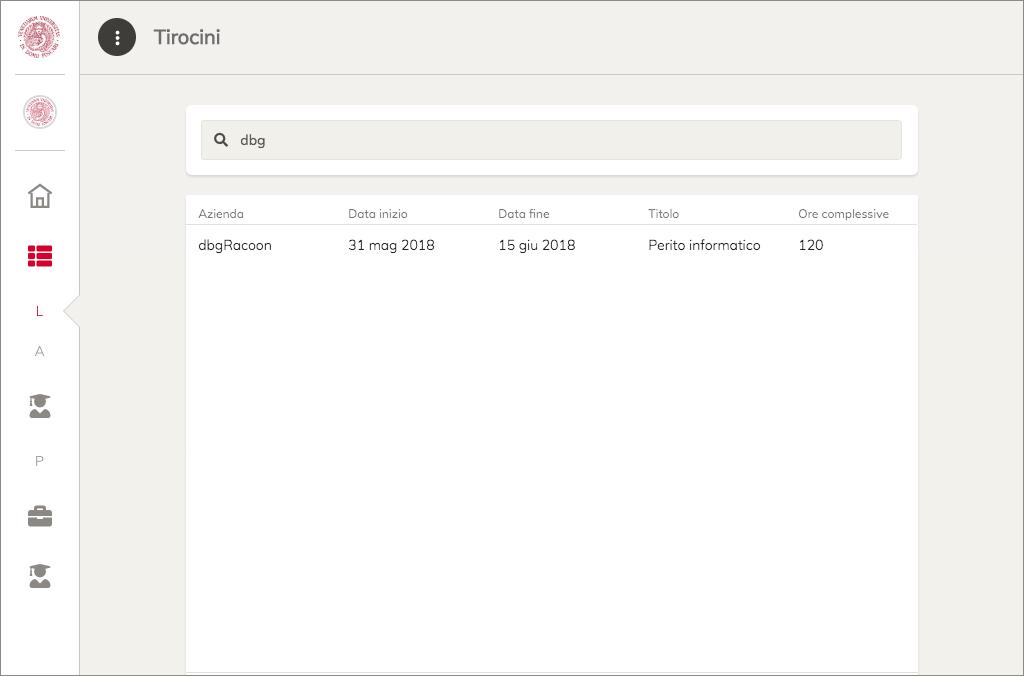
\includegraphics[width=\textwidth]{Chapter2/Figs/md-closed}     
		\caption{Sidebar collassata}
		\label{fig:screenshot:11}
	\end{subfigure}        
\end{figure}

\begin{figure}[h]\ContinuedFloat
	\centering
	\begin{subfigure}[b]{0.8\textwidth}
		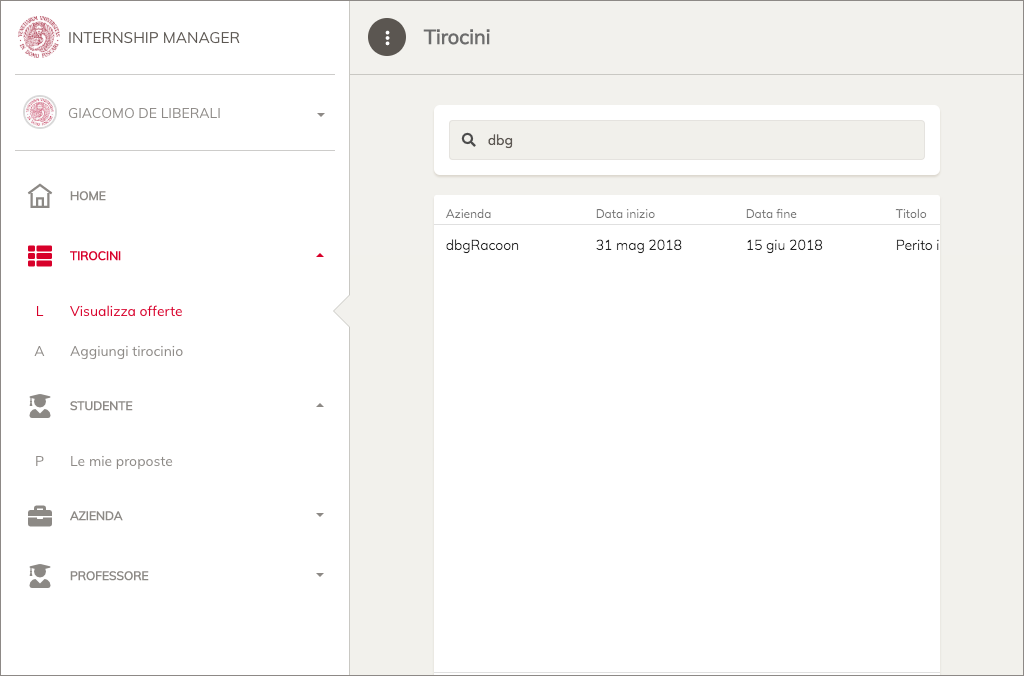
\includegraphics[width=\textwidth]{Chapter2/Figs/md-open}     
		\caption{Sidebar non collassata}
		\label{fig:screenshot:12}
	\end{subfigure}  
	\caption[Screenshot: layout del sistema in un tablet]{Layout del sistema in un tablet}
	\label{fig:screenshot:11-12}
\end{figure}

\begin{figure}[H]
	\centering
	\begin{subfigure}[b]{0.4\textwidth}
		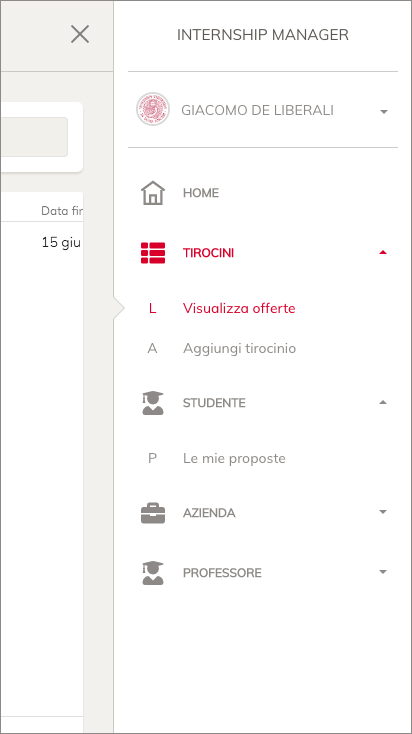
\includegraphics[width=1\textwidth]{Chapter2/Figs/xs-open}     
		\caption{Sidebar non collassata}
		\label{fig:screenshot:13} 
	\end{subfigure}        
	\hfil
	\begin{subfigure}[b]{0.4\textwidth}
		
\includegraphics[width=1\textwidth]{Chapter2/Figs/xs-closed}     
		\caption{Sidebar collassata}
		\label{fig:screenshot:14}
	\end{subfigure}  
	\caption[Screenshot: layout del sistema in uno smartphone]{Layout del sistema in uno smartphone}
	\label{fig:screenshot:13-14}
\end{figure}